\documentclass[fontsize=13pt]{scrartcl}
\usepackage[utf8]{vietnam}
\usepackage{amssymb}
\usepackage{amsmath}
\usepackage{algorithm}
\usepackage{longtable}
\usepackage{float}
\usepackage{url}
\usepackage{subfig}
\usepackage{algorithmic}
\usepackage[pdftex]{graphicx}
\usepackage{epstopdf}
\usepackage{multirow}
\usepackage{hhline}
\usepackage{setspace}
\usepackage{fancybox}
\usepackage{array}
\usepackage{longtable}
\usepackage{pgfplots}
\usepackage{float}
\usepackage{cite}
\usepackage{caption}
\usepackage{listings}
%\usepackage{biblatex}
%\addbibresource{ref.bib}
%\usepackage{hyperref}
%\pgfplotsset{compat = 1.10}

\renewcommand{\arraystretch}{1.5}
\makeatletter
\renewcommand{\ALG@name}{Thuật toán}
\makeatother
\usepackage{tabulary}
\renewcommand{\algorithmicrequire}{\textbf{Input:}}
\renewcommand{\algorithmicensure}{\textbf{Output:}}
\usepackage[newcommands]{ragged2e}
\usepackage[top=2cm, bottom=3.5cm, left=3.5cm, right=2cm]{geometry}
\renewcommand{\baselinestretch}{1.2}
\usepackage{lastpage}
\setcounter{page}{3}
\usepackage{fancyhdr}
\pagestyle{fancy}
\newcommand{\bigCI}{\mathrel{\text{\scalebox{1.07}{$\perp\mkern-10mu\perp$}}}}
\lhead{}
\chead{\thepage}
\rhead{}
\renewcommand{\footrulewidth}{0.4pt}
\lfoot{\small{Sinh viên thực hiện: Nguyễn Đức Anh, 20111119, K56, Lớp KSTN-CNTT}}
\cfoot{}
\rfoot{}
\begin{document}
\newpage
\begin{center}
\textbf{Lời Cảm Ơn}
\end{center}
Đầu tiên, em xin được gửi lời cảm ơn chân thành đến các thầy giáo, cô giáo thuộc trường đại học Bách Khoa Hà Nội. Đặc biệt là các thầy giáo, cô giáo thuộc Viện Công nghệ Thông tin và Truyền Thông. Chính các thầy cô giáo đã trang bị cho em những kiến thức quý báu trong thời gian em học tập và nghiên cứu tại trường. Đồng thời em cũng xin được gửi lời cảm ơn đặc biệt đến  PGS.TS Nguyễn Thị Kim Anh, TS Thân Quang Khoát, Ths Ngô Văn Linh. Các thầy cô là người đã chỉ dẫn tận tình, cho em những kinh nghiệm quý báu để em có thể hoàn thành đồ án tốt nghiệp này. Thầy cô luôn động viên, giúp đỡ em trong những thời điểm khó khăn nhất.
\par 
Em cũng xin gửi lời cảm ơn chân thành tới các thầy cô thuộc KDE lab thuộc Viện Công Nghệ Thông Tin và Truyền Thông đã tạo điều kiện cho em thực hành thử nghiệm trên các máy tính của lab.

Em xin gửi lời cảm ơn tới gia đình và bạn bè. Lời động viên tinh thần từ gia đình và bạn bè luôn là động lực để em tiến lên phía trước. 
\newpage
\begin{abstract}
\begin{center}
\textbf{Tóm Tắt Đồ Án}
\end{center}
Ngày nay với sự bùng nổ của internet, dữ liệu văn bản chữ ngày càng trở nên khổng lồ, việc phân tích thông tin từ lượng dữ liệu lớn này đã trở thành một bài toán khó thu hút nhiều sự quan tâm từ các nhà phân tích dữ liệu. Mô hình chủ đề, tiêu biểu là Latent Dirichlet Allocation (LDA)\textsuperscript{\cite{blei2003latent}} xuất hiện trong những năm gần đây đã tỏ ra như một phương pháp hiệu quả để xác định được cấu trúc ngữ nghĩa ẩn của dữ liệu văn bản nói chung và hứa hẹn nhiều ứng dụng. Để giải quyết các vấn đề về dữ liệu lớn trong điều kiện tài nguyên máy tính có hạn, các phiên bản học dòng cho LDA đã được tạo ra, tuy nhiên chúng đa phần đều chỉ sử dụng tri thức từ dữ liệu. Đồ án này đưa ra đề xuất việc đưa các tri thức về từ vựng từ bên ngoài vào quá trình học dòng cho mô hình LDA nhằm tăng khả năng tổng quát hóa cho mô hình. Các kết quả thử nghiệm trên 3 bộ dữ liệu Grolier, Nytimes và Pubmed cho thấy kết quả  phương pháp thử nghiệm tốt hơn về khả năng tổng quát so với mô hình học dòng cũ.
\end{abstract}
\newpage
\begin{abstract}
\begin{center}
\textbf{Abstract}
\end{center}
Nowadays, text data is become massive with the explosion of internet. The problem of analyzing information from these big data is a hard challenge which attract the concentration from many data analyst. Topic modeling such as Latent Dirichlet Allocation (LDA) has appeared in recent years and become an effective method to explore hidden semantic structure of documents. Streaming learning versions of LDA have been proposed to solve problem of massive data in condition of limiting computing resources but only focus on information from data. This thesis propose a method that give knowledge of vocabulary from other domains into learning process to improve the generalization capacity of model. The experiments on 3 data sets : Grolier, Nytimes and Pubmed showed that the results about the generalization capacity of proposal method are better than original LDA streaming model. 
\end{abstract}
\newpage 
\tableofcontents

\newpage
\textbf{Danh sách các từ viết tắt và thuật ngữ}

\begin{table}[H]
\begin{center}
\begin{tabular}{|l|l|}
\hline 
LDA & Latent Dirichlet Allocation \\
\hline 
pLSI & probabilistic Latent Semantic Analysis\\
\hline
Multinominal & Phân phối ngẫu nhiên đa thức\\
\hline
Dir & Phân phối Dirichlet \\
\hline
VB & Variational Bayesian \\
\hline
FW & Frank-Wolfe\\
\hline
Streaming learning & Học dòng\\
\hline
Online learning & Học trực tuyến\\
\hline 
Minibatch & Đoạn dữ liệu\\
\hline 
Train & Học - huyến luyện\\
\hline
Test & Kiểm tra\\
\hline
Topic & Chủ đề\\
\hline
Prior & Tri thức tiên nghiệm\\
\hline
Variational Inference & suy diễn biến phân \\
\hline
Variational distribution & Phân phối biến phân \\
\hline
Posterior distribution & phân phối hậu nghiệm \\
\hline
Prior distribution & Phân phối tiền nghiệm \\
\hline
Predictive Probability & Xác xuất tiên đoán\\
\hline
KP & Keeping prior: Phương pháp giữ tri thức tiên nghiệm\\
\hline
Origin & Nguyên bản\\

\hline 
\end{tabular}
\end{center}
\end{table}
\newpage
\textbf{Danh sách các kí hiệu dùng trong đồ án}
\begin{table}[H]
\begin{tabular}{|l|l|}
\hline
$\psi$ & hàm Digamma\\ \hline
$\Gamma$ & hàm Gamma \\ \hline
$\triangleq$ & kí hiệu cho "được định nghĩa là" \\ \hline
$K$ & số chủ đề sử dụng trong mô hình LDA \\ \hline
$V$ & kích thước từ vựng của tập văn bản\\ \hline
$\boldsymbol\beta $ & ma trận (K,V) mỗi hàng là xác suất của các từ trong mỗi chủ đề \\ \hline
$\boldsymbol\theta$ &vectơ tỷ lệ chủ đề trong mỗi văn bản \\ \hline
$w_n$ & từ thứ $n$ trong một văn bản \\ \hline
$z_n$ & chủ đề của từ thứ $n$ trong văn bản \\ \hline
$d_j$ & số lượng từ thứ j trong văn bản $d$\\ \hline
$\boldsymbol\eta $ & tham số của phân phối tiên nghiệm cho $\boldsymbol\beta$ \\ \hline 
$\boldsymbol\alpha$ & tham số của phân phối tiên nghiệm cho $\boldsymbol\theta$ \\ \hline
$\boldsymbol\gamma$ & tham số của phân phối biến phân ứng với $\boldsymbol\theta$ \\ \hline
$\boldsymbol\phi$ & tham số của phân phối biến phân ứng với $\mathbf{z}$ \\ \hline
$\boldsymbol\lambda$ & tham số của phân phối biến phân ứng với $\boldsymbol\beta$ \\ \hline
\end{tabular}
\end{table}

\newpage
\listoffigures 

\newpage
\listoftables
\newpage 
\section{Giới Thiệu Đề Tài}
Với sự bùng nổ của internet và máy tính điện tử, lượng dữ liệu văn bản chữ ngày càng trở nên khổng lồ với lượng tin tức hằng ngày từ các bài báo, các blog và các mạng xã hội. Việc phân tích thông tin từ khối lượng dữ liệu lớn này trở thành một vấn đề cấp thiết cho các nhà nghiên cứu dữ liệu. Bằng việc phân tích dữ liệu, các nhà nghiên cứu có thể rút ra được những lượng thông tin quý giá, chẳng hạn thói quen, sở thích hay xu hướng của người dùng, từ đó các công ty có những sách lược kinh doanh hợp lí. Tuy nhiên với lượng dữ liệu rất lớn tới hàng triệu văn bản, việc thống kê truyền thống bằng tay đã trở nên bất khả thi. Những mô hình học máy thống kê đã xuất hiện nhằm mục tiêu tự động phân tích ra cấu trúc dữ liệu với sự can thiệp hạn chế từ con người. Mô hình chủ đề, tiêu biểu là Latent Dirichlet Allocation (LDA) như một xu hướng mới đầy tiềm năng để phân tích cấu trúc ẩn bên trong của dữ liệu, đặc biệt là dữ liệu dạng văn bản chữ. Để giải quyết 3 vấn đề lớn:
\begin{itemize}
\item Lượng dữ liệu là cực kì lớn
\item Tài nguyên máy tính gồm bộ nhớ và vi xử lí là có hạn
\item Yêu cầu thời gian nhanh
\end{itemize} 
\par 
Các mô hình học trực tuyến và học dòng đã được đưa vào mô hình LDA. Cũng như mục tiêu ban đầu của học máy, việc học ra tham số của mô hình từ dữ liệu được thực hiện một cách tự động và giảm thiểu sự tác động của nhân tố con người. Các mô hình học cho LDA hiện tại đều chỉ lấy thông tin học từ dữ liệu, tuy nhiên với dữ liệu văn bản chữ, ta có một số thông tin hữu ích có được từ các nghiên cứu về ngôn ngữ, điển hình là 2 ví dụ sau:
\begin{itemize}
\item Tri thức về các từ thuộc một chủ đề cho trước. Bằng việc tìm hiểu về một miền chủ đề xác định, ta có thể đưa ra những từ đặc trưng tiêu biểu cho chủ đề. Ví dụ: về chủ đề thể thao, các từ: \textit{bóng đá, cầu thủ, bóng bàn, quần vợt, trận đấu…} là những từ đặc trưng cho chủ đề.
\item Các luật về ngôn ngữ, tiêu biểu là luật Zipf’s : Trong một văn bản chữ, tuần suất các từ xuất hiện tỉ lệ nghịch với hạng của từ trong bảng xếp hạng tần số của từ. Khi đó từ xuất hiện nhiều nhất sẽ có tần số xuất hiện xấp xỉ gấp đôi từ xuất hiện nhiều thứ 2…
\end{itemize}
\par 
Do vậy, khi phân tích các văn bản chữ, việc áp dụng các tri thức từ vựng này có thể nâng cao chất lượng học của mô hình. Đồ án này đề xuất việc đưa tri thức từ nhằm tăng khả năng tổng quát hóa cho quá trình học dòng của mô hình LDA. Những đóng góp của đồ án bao gồm:  
\begin{itemize}
\item Đưa tri thức từ vựng về dạng vector số để áp dụng vào mô hình học chủ đề.
\item Xây dựng công thức học dòng với sự tăng cường tri thức từ vựng cho mô hình học chủ đề.
\item So sánh và đánh giá với mô hình học dòng không có sự tăng cường tri thức từ vựng theo khả năng tổng quát hóa của mô hình.
\end{itemize} 
Bố cục của đồ án như sau: phần 2 giới thiệu những khái niệm về học cấu trúc ẩn và mô hình học chủ đề LDA, các dạng học toàn bộ, học trực tuyến và học dòng, phần này cũng nói về việc cần thiết của việc tăng cường tri thức trong học dòng. Phần 3 sẽ trình bày về công thức đề xuất cho quá trình học dòng có tăng cường tri thức bổ sung cho các mô hình học dòng nói chung và áp dụng cho mô hình LDA. Các kết quả thử nghiệm và đánh giá được trình bày trong phần 4. Phần 5 sẽ tổng kết lại đồ án và các định hướng tìm hiểu về sau.
\newpage
\section{Cơ sở lý thuyết}
\label{sec:partII}
	\subsection{Mô hình chủ đề}
	Trong phần ta sẽ trình bày các nội dung chính về mô hình chủ đề được sử dụng trong đồ án.
\subsubsection{Học chủ đề ẩn của dữ liệu văn bản chữ}
\textbf{\textit{Khái niệm chủ đề}}: Một chủ đề của dữ liệu có thể hiểu theo nghĩa thông thường, chẳng hạn chủ đề về thể thao, văn hóa hay chủ đề về chính trị, giáo dục…Căn cứ vào những từ xuất hiện trong văn bản mà ta có thể xác định văn bản đang nói về vấn đề gì. Nếu trong văn bản chứa các từ "tổng thống", "chủ tịch", "bầu cử", "cử tri", "đại biểu" , "nghị viện", " quốc hội" thì nó sẽ được xem là một văn bản nói về chính trị chứ không phải là thể thao. Như vậy một chủ đề được xác định bởi một tập hợp các từ đồng thời xuất hiện để làm nổi lên chủ đề đó trong một văn bản. Theo mặt toán học, mỗi chủ đề được biểu diễn bằng một phân phối các từ trong tập từ điển, các từ khác nhau. 
\par 
Một mô hình phân tích các chủ đề nằm trong dữ liệu nhằm mục tiêu học ra các chủ đề ẩn này.  Bằng việc xem xét cái văn bản dưới góc độ tổ hợp của các chủ đề ẩn, chúng ta có thể rút ra các đặc điểm của tập văn bản từ đó có nhiều ứng dụng như xác định các nội dung đặc trưng nằm trong tập văn bản, phân cụm các văn bản trong tập văn bản.
\par 
Học cấu trúc ẩn của dữ liệu, bắt đầu với mô hình phân tích ngữ nghĩa ẩn ( Latent Semantic Indexing - LSI) \textsuperscript{\cite{LSI}} và probabilitic Latent Semantic Indexing ( pLSI)\textsuperscript{\cite{plsi}} là lớp phương pháp học tại đó các văn bản và từ vựng được ánh xạ sang một không gian gọi là "không gian ngữ nghĩa ẩn"  hay được gọi là các "chủ đề ẩn". Trong một tập văn bản với D văn bản và V từ được mô tả trong ma trận $WORD_{[D\times V]}$, giả thiết có K chủ đề ẩn. Khi đó tập văn bản được chuyển sang không gian chủ đề ẩn là ma trận $DOC_{[D\times K]}$ trong đó mỗi văn bản sẽ bao gồm một tập các chủ đề ẩn. Các từ sẽ được chuyển sang không gian $TOPIC_{[K\times V]}$ trong đó mỗi chủ đề sẽ gồm một tập hợp các từ với tỉ lệ khác nhau.
\par

Phương pháp LSI đơn thuần sử dụng thuật toán tất định phân tách trị riêng nhằm tìm ra hai ma trận $DOC_{[D\times K]}$ và $TOPIC_{[K\times V]}$ sao cho $WORD_{[D\times V]} = DOC_{[D\times K]} * TOPIC_{[K\times V]} $. Mô hình pLSI tiến một bước dài hơn khi xem mỗi văn bản là tập hợp trộn của các chủ đề theo một phân phối cho trước và mỗi chủ đề ẩn sẽ là một phân phối xác xuất theo từ. Lúc này, việc tìm các tham số của mô hình ( gồm hai ma trận $DOC$ và $TOPIC$) để cực đại hóa xác xuất xảy ra của ma trận $WORD$:\\
\begin{center}max $probability(WORD | DOC, TOPIC)$\end{center}
Ta thấy rằng 2 mô hình LSI và pLSI đều có số lượng tham số trong ma trận $DOC$ tỉ lệ với số lượng văn bản có trong tập văn bản, việc tỉ lệ tuyến tính của tham số mô hình với kích thước dữ liệu sẽ dẫn tới gia tăng kích thước lưu trữ của mô hình. Ngoài ra cả 2 phương pháp đều cố định số lượng văn bản được học nên không có khả năng phân tích văn bản mới xuất hiện hoặc phải học lại tất cả từ đầu, đồng nghĩa với việc mô hình LSI và pLSI không có tính tổng quát hóa cho dữ liệu.
Để khắc phục những hạn chế này, mô hình LDA được đề xuất và đã đạt được những hiệu quả tốt.
\subsubsection{Mô hình LDA}
Phần này trình bày những kiến thức cơ bản về mô hình latent Dirichlet Allocation, được đề xuất bởi David M. Blei trong bài báo \textit{Latent Dirichlet allocation}\textsuperscript{\cite{blei2003latent}}. Chúng ta sẽ trình bày lại những điểm chính của mô hình được xem là đặt nền móng cho các mô hình chủ đề này.
\par
\textbf{\textit{1) Các khái niệm và kí hiệu}}
\begin{itemize}
\item Tập từ vựng gồm $V$ từ là đơn vị tạo thành văn bản.
\item Mỗi văn bản được kí hiệu là $d$
\item $d_j$ là số lần xuất hiện của từ $j$ trong văn bản.
\item Mỗi văn bản là một tập hợp của các từ $\textbf{w}= \{ w_1,w_2,…,w_N\}$ trong đó $w_i$ là từ thứ $i$ trong dãy các từ của văn bản. $N$ là số lượng từ trong văn bản. Mỗi văn bản được biểu diễn theo túi từ, khi đó ta chỉ quan tâm tới các từ xuất hiện mà không quan tâm tới thứ tự xuất hiện của nó trong văn bản.
\item Tập văn bản gồm $M$ văn bản $ D = \{\textbf{w}_1,\textbf{w}_2,...,\textbf{w}_M\}$ trong đó $\textbf{w}_i$ là văn bản thứ i trong tập văn bản.


\end{itemize}
\textbf{\textit{2) Mô hình sinh}}
\par
LDA là một mô hình sinh có xác suất của tập văn bản. Ý tưởng cơ bản là mỗi văn bản trong tập văn bản được trộn ngẫu nhiên bởi các chủ đề ẩn, mỗi chủ đề ẩn lại là một phân phối xác xuất của các từ, điều nay tương tự như mô hình pLSI. Tuy nhiên sự khác biệt của LDA với pLSI là ở chỗ, sự phân phối các chủ đề trong mỗi tập văn bản được giả định tuân theo một phân phối Dirichlet với tham số $\alpha$. Đặt $\beta$ là phân phối của các từ theo chủ đề ẩn. Để tăng tính tổng quát cho mô hình, phân phối các từ trong topic được giả thiết tuân theo phân phối Dirichlet với tham số $\eta$: $\beta \sim Dir(\eta)$. \\
Mô hình sinh được mô tả như sau:\\
Sinh tập các phân phối từ theo chủ đề.
\begin{enumerate}
\item Với mỗi chủ đề i trong ${1\ldots K}$
	\begin{enumerate}
		\item Lấy mẫu $\beta_i \sim Dir(\eta)$ 
	\end{enumerate}

\end{enumerate}
Sinh ra các từ của một văn bản
\begin{enumerate}
\item Chọn phân phối trộn các chủ đề của văn bản $\theta \sim Dir(\alpha)$
\item  Ứng với mỗi từ $w_n$ trong văn bản:
\begin{enumerate}
\item Chọn một chủ đề $z_n \sim Multinomial(\theta)$
\item Chọn ra từ $w_n \sim Multinomial(\beta_{z_{n}})$
\end{enumerate}
\end{enumerate}
Ở đây $\eta$ và $\alpha$ được gọi là các tri thức tiên nghiệm hay gọi là prior của phân phối Dirichlet. Mô hình LDA được biểu diễn bằng đồ thị xác xuất như hình (1) . Các kí hiệu mũi tên biểu diễn xác xuất có điều kiện. Các từ $w$ là đối tượng có thể quan sát được nên sẽ được tô đậm.
\begin{figure}[h]
\label{fig:ldaFull}
\begin{center}
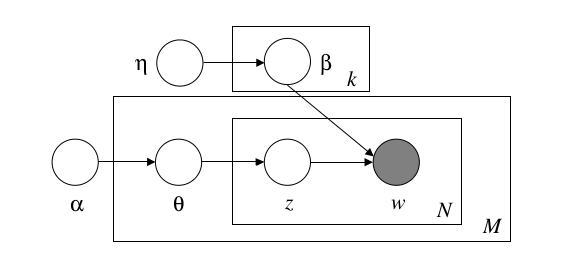
\includegraphics[scale=0.5]{img/lda_full.png}
\end{center}
\caption{Mô hình LDA}
\end{figure}
Như vậy mô hình LDA gồm có 3 phân mức: 
\begin{itemize}
\item Mức toàn cục: gồm các tham số $\eta, \alpha, \beta$ đặc trưng của mô hình cho tập dữ liệu
\item Mức văn bản: tham số $\theta$ xác định cho mỗi văn bản
\item Mức từ: Các chủ đề của mỗi từ $z$ cùng từ quan sát được $w$
\end{itemize}

Khi đó phân bố hợp của các biến ẩn $\boldsymbol\theta$, tập $N$ chủ đề $\mathbf{z}$ và tập $N$ từ $\mathbf{w}$ theo mô hình xác suất xác định bởi:
\begin{equation}
p(\boldsymbol{\theta},\mathbf{z},\mathbf{w},\boldsymbol\beta \mid \boldsymbol\alpha,\boldsymbol\eta) = p(\boldsymbol{\theta}\mid \boldsymbol\alpha )\prod_{n=1}^{N}p(z_n \mid \boldsymbol{\theta})p(w_n \mid z_n,\boldsymbol\beta)\prod_{k=1}^{K}p(\beta_k\mid \boldsymbol\eta)
\end{equation}
Trong đó:

\begin{align}
\boldsymbol\theta &\sim Dir(\boldsymbol\alpha)\\
p(z_n &= k\mid \boldsymbol\theta) = \theta_k\\
p(w_n\mid z_n &= k,\boldsymbol \beta) = \beta_{kw_n}\\
p(\beta_k \mid \boldsymbol\eta) & \sim Dir(\boldsymbol\eta) 
\end{align}
Xác suất xuất hiện của tập văn bản $\mathbf{w}$ với điều kiện là tham số mô hình $\alpha, \eta$ được xác đỉnh bằng tích phân trên miền giá trị $\theta, \beta$ và tổng trên $z$ của phân phối hợp:


\begin{equation}\label{eq:margin_dis}
p(\mathbf{w} \mid \boldsymbol{\alpha},\boldsymbol\eta)= \int_{\boldsymbol\beta}\int_{\boldsymbol\theta} p(\boldsymbol\theta \mid \boldsymbol\alpha)\big(\prod_{n=1}^{N}\sum_{z_n}p(z_n\mid \boldsymbol\theta) p (w_n\mid z_n,\beta) \prod_{k=1}^{K}p(\beta_k\mid \boldsymbol\eta) \big)d\boldsymbol\theta d\boldsymbol\beta
\end{equation}
Đây cũng chính là phân phối biên của văn bản. Mục tiêu của việc học mô hình từ dữ liệu nhằm cực đại hóa phân phối này. 
\subsubsection{Bài toán suy diễn cho mô hình LDA}\label{sub:infermethods}
Như trình bày ở trên, chúng ta cần những thuật toán xấp xỉ để tìm ra các tham số của mô hình nhằm tối ưu (\ref{eq:margin_dis}). Để giải quyết vấn đề này, chúng ta sử dụng thuật toán E-M với 2 bước:
\begin{enumerate}
\item Bước E: Giữ cố định các tham số $\alpha,\eta$ của mô hình, cập nhật các tham số ẩn $\theta,z$. Bước này cũng được gọi là bước suy diễn. Chúng ta gọi là suy diễn bởi sau khi có được văn bản, ta lại đi tìm các tham số để sinh ra văn bản.
\item Bước M: Giữ cố định các tham số của văn bản, cập nhật lại cái tham số toàn cục $\alpha,\eta,\beta$
\end{enumerate}
Bước suy diễn có thể viết lại về hàm phân phối xác xuất:
\begin{equation}
p(\boldsymbol\theta,\mathbf{z},\boldsymbol\beta \mid \mathbf{w},\alpha,\eta) = \frac{p(\boldsymbol\theta,\mathbf{z},\mathbf{w},\boldsymbol\beta \mid \alpha,\eta)}{p(\mathbf{w},\alpha,\eta)}
\end{equation}
Việc giải trực tiếp vấn đề tối ưu của phân phối này là điều không khả thi \textsuperscript{\cite{intract}}, vì vậy chúng ta cần sử dụng những phương pháp xấp xỉ. Sau đây là 3 phương pháp được sử dụng trong đồ án để giải quyết bài toán suy diễn.\\ 
\textbf{\textit{1. Phương pháp biến phân }}
\par 
Phương pháp suy diễn biến phân cho mô hình LDA được trình bày trong bài báo gốc \textit{Latent Dirichlet Allocation}\textsuperscript{\cite{blei2003latent}}.
Ở phương pháp này, thay vì tìm cực đại của hàm, chúng ta sẽ tìm một cận dưới của nó bằng bất đẳng thức Jensen rồi sau đó tìm cực đại của hàm cận dưới này bằng cách xem xét các biến dưới một miền phân phối định trước.
Trở lại hàm phân phối hậu nghiệm $\log p(\mathbf{w}|\alpha,\eta)$ ( Sử dụng hàm $\log$ để dễ tính toán). Áp dụng bất đẳng thức Jensen ta có:
\begin{align}
\log p(\mathbf{w} | \alpha, \eta) &= \log \int \sum_{z} p(\theta,\mathbf{z},\mathbf{w},\beta | \alpha,\eta)d\theta d\beta \\
&= \log \int \int \sum_{z} \frac{p(\theta,\mathbf{z},\mathbf{w},\beta | \alpha,\eta)q(\theta,\mathbf{z},\beta)}{q(\theta,\mathbf{z},\beta)} \\
&\geq \int\int\sum_{z}q(\theta,\mathbf{z},\beta)\log p(\theta,\mathbf{z},\mathbf{w},\beta | \alpha,\eta) d\theta d\beta - \int\int\sum_{z}q(\theta,\mathbf{z},\beta) d\theta d\beta\\
&=E_q (p(\theta,\mathbf{z},\mathbf{w},\beta | \alpha,\eta)) - E_q(q(\theta,\mathbf{z},\beta)) \label{eq:varialeft}
\end{align}
Ở đây $q(\theta,\textbf{z},\beta) $ là phân phối biến phân. Xét các họ biến phân:
\begin{equation}
q(\theta,\textbf{z},\beta) = q(\theta)q(\textbf{z})q(\beta)
\end{equation}
Trong đó:
\begin{align}
q(\theta) &= Dir(\theta|\gamma)\\
q(\mathbf{z}) &= \prod_{n=1}^{N} q(z_n|\phi_n)\\
q(\beta) &= Dir(\beta | \lambda)
\end{align}

Đặt vế trái của (\ref{eq:varialeft}) là $L(\gamma,\phi,\lambda;\alpha,\eta)$. Ta viết phân phối hậu nghiệm dưới dạng:
\begin{equation}
\log p(\mathbf{w} | \alpha, \eta) = L(\gamma,\phi,\lambda;\alpha,\eta) + D(q(\theta,\mathbf{z},\beta| \gamma,\boldsymbol\phi,\lambda) || p(\theta,\mathbf{z},\beta | \alpha,\eta,\mathbf{w}))
\end{equation} 
\begin{figure}[H]
\begin{center}
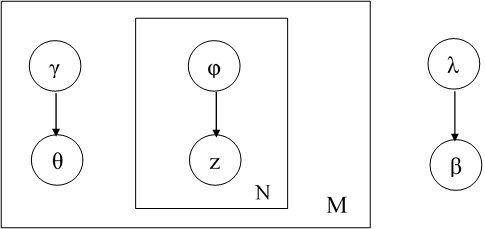
\includegraphics[scale=0.6]{img/variationalinfer.png}
\end{center}
\label{fig:variationalinfer}
\caption{Suy diễn biến phân cho mô hình LDA}
\end{figure}
Hàm $L(\gamma,\phi,\lambda;\alpha,\eta)$ chính là hàm chặn dưới cho phân phối hậu nghiệm, còn được gọi là ELBO ( \textbf{E}vidence \textbf{L}ower \textbf{BO}und ). $D(q(\theta,\mathbf{z},\beta| \gamma,\boldsymbol\phi,\lambda) || p(\theta,\mathbf{z},\beta | \alpha,\eta,\mathbf{w})$ là khoảng cách Kullback–Leibler của 2 phân phối $q(\theta,\mathbf{z},\beta| \gamma,\boldsymbol\phi,\lambda)$ và $p(\theta,\mathbf{z},\beta | \alpha,\eta,\mathbf{w})$\\
Việc cực đại hóa $L$ đồng nghĩa với việc giảm khoảng cách $D$ khiến phân phối  $q(\theta,\mathbf{z},\beta| \gamma,\boldsymbol\phi,\lambda)$ càng gần với phân phối $p(\theta,\mathbf{z},\beta | \alpha,\eta,\mathbf{w})$.\\
Chính vì vậy  $q(\theta,\mathbf{z},\beta| \gamma,\boldsymbol\phi,\lambda)$ được gọi là phân phối biến phân của $p(\theta,\mathbf{z},\beta | \alpha,\eta,\mathbf{w})$
\par 
Khai triển $L(\gamma,\phi,\lambda;\alpha,\eta)$ theo mô hình xác xuất của LDA
\begin{equation}
\begin{split}
 \mathcal{L}(\mathbf{w},\boldsymbol\phi, \boldsymbol\gamma,\boldsymbol\beta) = 
\sum_d \{ \mathbb{E}_q[\log p(w_d \mid z_d,\boldsymbol\beta)] + \mathbb{E}_q[\log p(z_d\mid \theta_d)]  -\mathbb{E}_q[\log q(z_d)] + \\ \mathbb{E}_q[\log p(\theta_d \mid \alpha)] - \mathbb{E}_q[\log q(\theta_d)]  +(\mathbb{E}_q[\log p(\boldsymbol\beta \mid \eta)] - \mathbb{E}_q[\log q(\boldsymbol\beta)])/M \}
\end{split}
\end{equation}
Tiếp tục biến đổi ta có:
\begin{equation}
\begin{split}
\mathcal{L} = \sum_{d}\sum_{w}n_{dk}\sum_{k}\phi_{dwk}(\mathbb{E}_{q}[\log\theta_{dk}] +\mathbb{E}_q[\log\beta_{kw}] - \log\phi_{dwk} ) \\
- \log\Gamma(\sum_{k}\gamma_{dk}) + \sum_{k}(\alpha - \gamma_{dk})\mathbb{E}_q[\log \theta_{dk}] + \log\Gamma(\gamma_{dk})\\
+(\sum_{k} -\log\Gamma(\sum_{w}\lambda_kw) + \sum_{w}(\eta - \lambda_{kw})\mathbb{E}_q[\log\beta_{kw}] + \log\Gamma(\lambda_{kw}))/D\\
+ \log\Gamma(K\alpha) - K\log\Gamma(\alpha) + (\log\Gamma(V\eta) - W\log\Gamma(\eta))/M
\end{split}
\end{equation}
Trong đó $V$ là kích thước của tập từ vựng và $M$ là số văn bản trong tập văn bản. $l(n_d,\phi_d,\gamma_d,\boldsymbol\lambda)$ kí hiệu phần đóng góp của văn bản $d$ vào ELBO. Cực đại $\mathcal{L}$ theo các tham số tự do của phân phối $q$, bằng cách tính đạo hàm theo từng tham số ta có được các công thức cập nhật:
\begin{align}
\phi_{dwk} &\propto exp\{\mathbb{E}_q[\log\theta_{dk}] + \mathbb{E}_q[\log\beta_{kw}]\} \label{eq:variantphi}\\
\gamma_{dk} &= \alpha + \sum_{w}n_{dk}\phi_{dwk} \label{varaintgamma}\\
\lambda_{kw} &= \eta + \sum_{d}n_{dw}\phi_{dwk} 
\end{align}
Các giá trị kì vọng:
\begin{align}
\mathbb{E}_q[\log\theta_{dk}] &= \Psi(\gamma_{dk}) - \Psi(\sum_{i=1}^{K}\gamma_{di})\\
\mathbb{E}_q[\log\beta_{kw}] &= \Psi(\lambda_{kw}) - \Psi(\sum_{i=1}^{W}\lambda_{ki})
\end{align}
Kí hiệu $\Psi$ được sử dụng là hàm digamma. \\
Các công thức (\ref{eq:variantphi}) và (\ref{varaintgamma}) chính là các công thức suy diễn thông tin cho mỗi văn bản $d$.
\par
Như vậy với phương pháp biến phân, chúng ta không tìm được trực tiếp giá trị của các tham số trong mô hình ban đầu nhưng tìm được các biến phân của chúng. Đây có thể xem như là một không gian con cho các phân phối của các tham số trong mô hình. Việc sử dụng biến phân như trình bày ở trên sẽ giới hạn không gian tìm kiếm của các tham số trong miền biến phân. Do vậy kết quả tìm được có thể không phải là tối ưu toàn cục, để mở rộng không gian tìm kiếm hơn, phương pháp suy diễn sử dụng thuật toán Frank-Wolfe được đề xuất trong các bài báo \textit{Fully sparse topic models} \cite{fullyspared}, \textit{Inference in topic models i : sparsity and trade-off}\cite{fwinfer}, \textit{Dual online inference for latent Dirichlet Allocation} \cite{dualonline}, đã thể hiện đem lại hiệu quả cao hơn về chất lượng hàm tối ưu.

\par
\textbf{\textit{2. Phương pháp suy diễn Frank-Wolfe}}\\
Phương pháp này sử dụng thuật toán Frank-Wolfe để tối ưu hàm lồi. Lúc này giá trị tham số $\alpha$ được đặt bằng 1. Hàm phân phối hậu nghiệm trở thành một hàm lồi. Việc tìm giá trị của tham số sẽ không cần dùng biến phân, và do đó có thể trực tiếp tìm ra giá trị $\theta$. Giả định rằng giá trị $\beta$ đã được tính trước. Cần tính ra giá trị $\theta$ của văn bản $d$ với hàm cần tối ưu $f(\theta)= \sum_{j}d_{j}log\sum_{k=1}^{K}\theta_{k}\beta_{kj}$. Thuật toán được mô tả như sau:
\begin{algorithm}[H]
\begin{algorithmic}
\caption{Thuật toán suy diễn Frank-Wolfe}
\label{frankwolfeInfer2}
\REQUIRE{ Văn bản $d$, tham số $\beta$}
\ENSURE{$\theta$\\}
Lấy $\theta_0$ tại một đỉnh $\Delta_K$ của hàm  $f(\theta)= \sum_{j}d_{j}log\sum_{k=1}^{K}\theta_{k}\beta_{kj}$ \\
\FOR { $l = 1,...,\infty$}
\STATE {$i' \leftarrow argmax_{i}\bigtriangledown(f(\theta_l)_i$}
\STATE {$\alpha \leftarrow 2/(l+3)$}
\STATE{$\theta_{l+1} \leftarrow \alpha.e_{i'} + (1-\alpha)\theta_l$}
\ENDFOR
\STATE $\theta^{*} \leftarrow _{\theta_l} max f(\theta_l)$
\end{algorithmic}
\end{algorithm}
Ta kí hiệu:
\begin{equation}
	\theta \leftarrow FW(\beta,d)
\end{equation} 
Việc đặt giá trị $\alpha = 1$ làm thiếu tính tổng quát của mô hình, đồng thời cũng thể hiện rõ thuật toán suy diễn Frank-Wofle không giải quyết được những hàm không lồi khi $\alpha != 1$. Để giải quyết điều này ta dùng thuật toán suy diễn Online Frank-Wolfe
\par
\textbf{\textit{3. Phương pháp Online Frank-Wolfe}}\\
Ở phương pháp này, hàm không lồi được chia thành hai phần, hàm cần tối ưu là hàm tổng ngẫu nhiên của một trong hai thành phần với xác suất bằng nhau. Thuật toán được mô tả chi tiết như sau:
\begin{algorithm}[H]
\begin{algorithmic}
\caption{Thuật toán suy diễn Online Frank-Wolfe}
\label{onlfrankwolfeInfer}
\REQUIRE{ Văn bản $d$, tham số $\beta,\alpha$}
\ENSURE{$\theta$\\}
%Pick as $\theta_0$ the vertex of $\Delta_K$ over  $f(\theta)= \sum_{j}d_{j}log\sum_{k=1}^{K}\theta_{k}\beta_{kj}$ \\
Khởi tạo $\theta$ thuộc $\Delta_{K} = {x \in R^{K} : \sum_{k=1}^{K} x_k = 1, x_k>0}$
\FOR {$l = 1,...,\infty$}
\STATE{Lấy $f_l$ ngẫu nhiên đều nhau từ \{${\sum_{j}d_{j}log\sum_{k=1}^{K}\theta_{k}\beta_{kj};(\alpha-1)\sum_{k=1}^{K}log\theta_k}$\}}
\STATE{$F_l \leftarrow 2/l$}\\
\STATE{$i' \leftarrow argmax_{i} \nabla F_{l}(\theta_l)_i)$}\\
\STATE{$\zeta \leftarrow 1/ \sqrt{l}$}
\STATE{$\theta_{l+1} \leftarrow \zeta.\textbf{e}_{i'} + (1-\zeta)\theta_l$}
\ENDFOR
\end{algorithmic}
\end{algorithm}
Ta kí hiệu 
\begin{equation}
\theta \leftarrow OFW(\beta,\alpha,d)
\end{equation}

Các chứng minh đã chỉ ra thuật toán Online-Frankwolfe có tốc độ hội tụ và chất lượng hàm tối ưu hơn FW và VB. Tuy nhiên cả Frank-Wolfe và Online Frank-Wolfe đều chưa trực tiếp tính ra được tham số của các chủ đề của từ trong văn bản $z$. Song chúng ta có thể suy diễn ra nó từ tính chất của mô hình
\begin{equation}
\phi_{jk} = p(z = k | w = j, d)
\end{equation}
Từ đó rút ra được:
\begin{equation}
\phi_{jk} \sim \theta_{k}\beta_{kj}
\end{equation}

\subsubsection{Vấn đề cập nhật các tham số toàn cục}
Các tham số toàn cục $\alpha,\eta$ mặc dù có phương pháp cập nhật thông qua bước M-Step. Tuy nhiên điều này sẽ làm tăng thêm tính phức tạp và thời gian thực hiện của quá trình học mô hình. Trên thực tế cài đặt, các tham số này được giữ cố định bởi một giá trị nhỏ hơn 1. Trong điều kiện không có tri thức về ữ liệu, để đảm bảo tính cân bằng, các tham số này là các tham số đối xứng ( các giá trị bằng nhau) của phân phối Dirichlet. Việc đặt giá trị nhỏ hơn 1 bởi tính chất thưa trong văn bản, khi mỗi văn bản thường chỉ có một số chủ đề xác định và mỗi chủ đề thông thường cũng chỉ tập trung ở một số từ chứ không trải đều. Điều này phù hợp với tính chất của phân phối Dirichlet với các tham số nhỏ hơn một, các giá trị của phân phối tập trung ở một số đỉnh thay vì trải đều trên miền xác định. Vì vậy đồ án này đề cập tới vấn đề cập nhật khi các tham số phân phối tiên nghiệm được đặt cố định.
\par
Xét riêng ở phân phối của các từ theo chủ đề $\beta \sim Dir(\eta)$. Ta nhận thấy rằng, nếu có trước các tri thức về phân phối các từ đặc trưng cho bộ dữ liệu, chúng ta có thể nâng cao chất lượng cho $\beta$.  Từ nhận xét này, ta sẽ kết hợp tri thức từ và đưa vào mô hình học chủ đề LDA bằng cách cung cấp nó vào tham số $\eta$ với mục đích nâng cao chất lượng học của mô hình. Từ đây,  tri thức tiên nghiệm của mô hình LDA được gọi riêng cho $\eta$ - tri thức có trước về phân phối các từ trong chủ đề.  
\subsection{Các dạng học cho mô hình chủ đề}
Phần này đề cập tới 3 phương pháp học dữ liệu dựa trên khía cạnh phân chia dữ liệu đầu vào.
\subsubsection{Học toàn bộ dữ liệu}
\begin{figure}[h]
\begin{center}
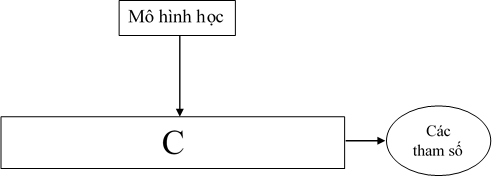
\includegraphics[scale=0.7]{img/batch.png}
\end{center}
\label{fig:batchLearning}
\caption{Phương pháp học batch}
\end{figure}
Học toàn bộ dữ liệu hay còn gọi là học batch\textsuperscript{\cite{blei2003latent}} (hình 3). Trong phương pháp học này, toàn bộ dữ liệu được sử dụng để học ra tham số của mô hình. Trong các vòng lặp của quá trình học, toàn bộ dữ liệu được sử dụng lại. Điều này rất tốn kém về bộ nhớ cũng như thời gian thực hiện, do vậy là không khả thi cho trường hợp dữ liệu lớn.
\subsubsection{Học trực tuyến}
\begin{figure}[h]
\begin{center}
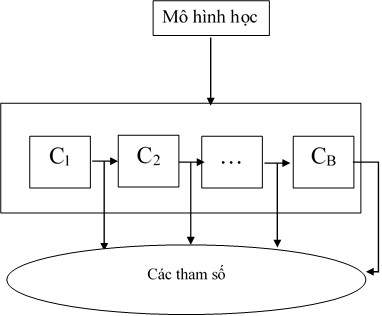
\includegraphics[scale=0.7]{img/online.png}
\end{center}
\label{fig:onlineLearning}
\caption{Phương pháp học trực tuyến - online}
\end{figure}
Học trực tuyến - hay học online\textsuperscript{\cite{onlineLDA}} (hình 4), dữ liệu ban được chia ra làm các đoạn nhỏ, việc hoc tham số mô hình được thực hiện thông qua việc học từ các đoạn dữ liệu nhỏ này. Như vậy quá trình học sẽ không phải sử dụng toàn bộ dữ liệu và thăm lại dữ liệu đã học qua nên tiết kiệm được chi phí tài nguyên bộ nhớ và thời gian. Tuy nhiên phương pháp học này cần thực hiện trên không gian dữ liệu đã xác định kích thước, do vậy là khó thực hiện với dữ liệu tới liên tục.
\subsubsection{Học dòng}\label{subsec:streamingintro}
\begin{figure}[h]
\begin{center}
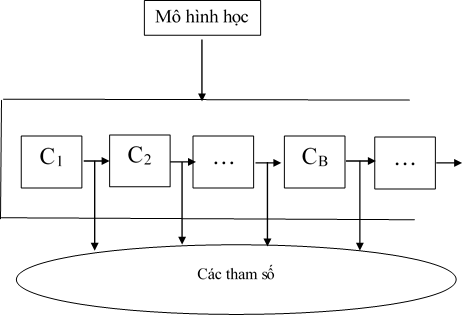
\includegraphics[scale=0.7]{img/streaming.png}
\end{center}
\label{fig:streamingLearning}
\caption{Phương pháp học dòng - streaming}
\end{figure}
Học dòng giải quyết được cả 2 vấn đề mà học batch và học online gặp phải bằng việc học liên tiếp các đoạn dữ liệu tới mà không cần thăm lại dữ liệu đã học qua cũng như cần biết trước khối lượng dữ liệu (hình 5). Do vậy học dòng sẽ thích hợp với việc phân tích dữ liệu lớn, đây là lí do mà đồ án này lựa chọn phương pháp học dòng để phát triển cho mô hình LDA.\\
Đề cập sâu hơn về học dòng, một mô hình học dòng tổng quát được đề xuất bởi Tamara Broderick và cộng sự trong bài báo \textit{Streaming variant Bayes}\textsuperscript{\cite{streamvb}}. Chúng ta sẽ trình bày các điểm chính trong phương pháp học dòng này.\\
\textit{1. Các khái niệm và kí hiệu}
\begin{itemize}
\item Dãy các văn bản thu thập được xem được biểu diễn bởi một dòng các văn bản $d_1, d_2, \ldots$ 
\item Các văn bản được thu tập thành dãy các đoạn – minibatch C, mỗi minibatch sẽ bao gồm một tập hợp các văn bản, các batch khác nhau sẽ không có chung văn bản.  
\item Dòng dữ liệu S sẽ là dãy các Batch thu thập được $S = \{ C_1, C_2, \ldots \}$
\item Mô hình sinh của các văn bản được xác định theo tham số $\Phi$. Một tri thức tiên nghiệm về phân phối các từ được đưa vào $\eta$.
\end{itemize}
\textit{2. Mô hình học dòng không tăng cường tri thức tiên nghiệm}\\
Giả định rằng ta đã nhận được lượng dữ liệu từ $B-1$ minibatch với thông tin xử lí được là xác suất hậu nghiệm: $p(\Phi | C_1,C_2,…C_{B-1} )$. Dữ liệu từ minibatch $C_B$ tới và mô hình cần được cập nhật.
Để giải quyết tìm tham só $\Phi$ mới, ta cần tìm $\Phi$ để tối đa hóa xác xuất $p(\Phi| C_1,C_2, …,C_B)$. Sử dụng biến đổi Bayes ta được:
\begin{equation}\label{eq:oldstream}
p(\Phi| C_1, C_2, \ldots,C_B) \propto p(C_B| \Phi)p(\Phi| C_1, C_2,\ldots, C_{B-1})
\end{equation}
Tuy nhiên việc tính chính xác các phân phối này thường là không khả thi, vì vậy cần những phương pháp xấp xỉ. 
Giả định rằng cho trước $p(\Phi)$ với dữ liệu $C$, $A$ là một thuật toán xấp xỉ để tính $p(\Phi)$ với $q(\Phi) = A(C,p(\Phi))$. Đặt $q_0(\Phi) = p(\Phi)$. Do $p_B(\Phi) \approx q_B(\Phi)$ nên ta được:
\begin{equation}
p(\Phi | C_1,C_2,\ldots,C_{B-1},C_B) \approx q_B(\Phi) = A(C,q_{B-1}(\Phi))
\end{equation}
Phân tách dòng dữ liệu thành các chuỗi minibatch:
\begin{equation}
p(\Phi | C_1,…,C_B ) \propto [ \prod_{b=1}^{B} p(C_b |  \Phi )]p(\Phi) \propto [\prod_{b=1}^{B} p(\Phi | C_b) p(\Phi)^{-1}]p(\Phi)]
\end{equation}
Tiếp tục áp dụng xấp xỉ, ta được
\begin{equation}\label{eq:oldstreamupdate}
p(\Phi |C_1,...,C_B) \approx q(\Phi) \propto [\prod_{b=1}^{B} A(C_b,p(\Phi)) p(\Phi)^{-1}]p(\Phi)
\end{equation}
Như vậy bằng việc lấy thông tin học được từ $B-1$ minibatch trước, kết hợp thông tin hiện tại, chúng ta đã hoàn toàn học được thông tin cho mô hình với tất cả dữ liệu có được mà không cần  duyệt lại thông tin trước đó. Hơn thế, việc các minibatch có thể tính độc lập giúp cho việc học có thể thực hiện song song trên các đoạn dữ liệu, nhờ đó tăng tốc độ học.
\subsubsection{Sự cần thiết của bổ sung tri thức vào quá trình học dòng}
Theo công thức cập nhật ở \ref{eq:oldstream}, chúng ta thấy có hai vấn đề:
\begin{itemize}
\item Vai trò tham số tiên nghiệm - prior cho dữ liệu chưa được đề cập. Toàn bộ lượng thông tin học được đều có được từ dữ liệu.
\item Phân phối hậu nghiệm (posterior) từ lượng dữ liệu đã học được sử dụng như phân phối tiên nghiệm (prior) cho minibatch mới đến, bằng cách học liên tục này, những thông tin cung cấp từ tri thức tiên nghiệm sẽ nhanh chóng bị "mờ" đi theo thời gian.\\
Như vậy khi có được tri thức tiên nghiệm, bên cạnh việc cung cấp vào mô hình học dòng, chúng ta cần phải tăng cường nó để tránh bị "mờ" đi trong quá trình học. Điều này sẽ được trình bày chi tiết trong phần 3. Trước đó chúng ta chúng ta sẽ tìm hiểu một số tri thức về từ vựng có thể sử dụng làm tri thức tiên nghiệm.
\end{itemize}
\subsection{Tri thức từ vựng}\label{sub:wordknowledge}
Chúng ta sẽ đề cập tới hai tri thức có được bên ngoài dữ liệu, đó là các từ đặc trưng theo chủ đề và luật Zipfs của ngôn ngữ. 
\subsubsection{ Các từ đặc trưng của chủ đề}
Khi đề cập tới một chủ đề, chúng ta có thể xác định được một số từ đặc trưng cho chủ đề đó hoặc các từ xuất hiện nhiều theo chủ đề. Chẳng hạn trong chủ đề thể thao, nói về thể thao các từ \textit{ cầu thủ, bóng đá, bóng bàn, cầu lông, \ldots }sẽ phản ảnh được chủ đề đang đề cập.
\par
Một cách tổng quát, khi các nhà nghiên cứu tìm hiểu về một chủ đề tri thức xác định ( domain knowledge), chúng ta có thể rút ra được những từ ngữ đặc trưng cho chủ đề (seed-words). Các từ này xuất hiện như một dấu hiệu để nhận biết chủ đề bao chứa. Bảng \ref{tb:topicword} minh họa một số từ chủ đề thuộc 3 topic Công nghệ, Sinh học, Thể thao. ( Nguồn: myvocabulary.com/wordlist\textsuperscript{\cite{listwordtopic}})

\textbf{}
%\begin{table}[H]
\begin{center}
\begin{longtable}{| p{.2\textwidth} | p{0.8\textwidth} |}

\hline 
Chủ đề công nghệ \newline (Technology) & Access, Account, Activity, Administrative, Advantage, Advertisements, Animate, Applications, Back up, Bandwidth, Banner, Camera, Capabilities, Capacity, Capture,  E-mail, Edit, Educate, Effective, Efficiency, Face Book, Fax, Fiber optic, Field, Telecommunication, Telemarketer, Telephone, Television, Terminal, Warranty, Wave, Web master, Web page, Web site, Windows, Wireless, Word   \\
\hline
Chủ đề sinh học \newline (Biology) & Absorption, Achromatic, Adaptation, Aerobic, Algae, Alimentary, Allergy, Backbone, Bacteria, Balance, Barrier, Benign, Biology, Biome, Ecology, Ecosystem, Ectoplasm, Edema, Embryo, Endangered, Endemic, Factor, Feedback, Fertilization, Fetus, Fibrillation, Filament, Fish, Natural, Nerve, Neuron, Nitrogen, Scope, Secrete, Seed, Sensor, Shelter, Skeleton, Skin,  Stress, Structure, Symbiosis,  Y chromosome  \\
\hline
Chủ đề thể thao \newline (Sport) & Acrobatics, Aerobics, Aikido, Badminton, Baseball, Basketball, Beach volleyball, Cycling, Golf, Gymnastics, Olympics, Open water swimming, Table tennis, Table tennis, Tae Kwon Do, Target shooting, Tennis, Yachting, Yoga\\
\hline
\caption{Một số các chủ đề và các từ đặc trưng}
\label{tb:topicword}

\end{longtable}

\end{center}
%\end{table}
\subsubsection{Luật Zipf’s}
Luật Zip’s \textsuperscript{\cite{zipf2},\cite{zipflaw}} là một luật được rút ra từ thực nghiệm thông qua quá trình thống kê toán học. Luật được đề xuất bởi nhà ngôn ngữ học: George Kingsley Zipf. Luật Zipf’s được phát biểu như sau:\\[0.4cm]
\fbox{\begin{minipage}{0.9\textwidth}
Trong một tập văn bản của một ngôn ngữ tự nhiên, tần số xuất hiện của các từ tỉ lệ nghịch với hạng của nó trong bảng xếp hạng tần số của từ.
\end{minipage}}
\\[.4cm]
 Công thức toán học của luật:
\begin{equation}
f(k;s,N) = \frac{1/k^s}{\sum_{n=1}^N(1/n^s)}
\end{equation}
Hay viết lại dưới dạng:
\begin{equation}
f(k;s,N) = \frac{1}{k^sH_{N,s}}
\end{equation}
Trong đó:
\begin{center}
\begin{itemize}
\item $N$ là số lượng từ
\item $k$ là hạng của từ trong bảng xếp hạng tần số
\item $s$ là giá trị tùy thuộc vào loại ngôn ngữ
\item $H_{N,s}$ là hàm Harmonic tổng quát bậc s của phần tử N.
\end{itemize}
\end{center}

Luật Zip được tổng quát hóa hơn bởi luật Zipf-mandelbro, đề xuất bởi Benoit Mandlbrot, khi đó tần suất của từ xác định bởi
\begin{equation} \label{eq:zipfman}
f(k;N,q,s) = \frac{[constant]}{[k+q]^s}
\end{equation}
Bằng xấp xỉ Yule-Simon cho (\ref{eq:zipfman}), ta được công thức xấp xỉ rút gon:
\begin{equation}\label{eq:zipex}
f(k;p) \approx \frac{[constant]}{k^{p+1}}
\end{equation}
Ở đây $s$ là hằng số $>1$ và $q>0$
Trong tập tiếng anh  $q = 0.07$, giá trị hằng số tùy thuộc vào văn bản.
\par
Hai dạng tri thức từ vựng về các từ chủ đề và luật Zipfs có thể dễ dàng chuyển về dạng phân phối từ, do đó có thể cung cấp vào tri thức tiên nghiệm cho mô hình học chủ đề LDA.


\newpage
\section{Tăng cường tri thức tiên nghiệm vào quá trình học dòng}
Phần này sẽ trình bày đề xuất của đồ án về phương pháp học dòng tổng quát với sự tăng cường của tri thức tiên nghiệm. Phương pháp được áp dụng cụ thể cho mô hình LDA.
\subsection{Phương pháp học dòng với tri thức tiên nghiệm tăng cường}
Ý tưởng cơ bản của đề xuất này nằm ở việc liên tục bổ sung tri thức tiên nghiệm cho mỗi minibatch cho quá trình học dòng (hình 6).
\begin{figure}[h]
\begin{center}
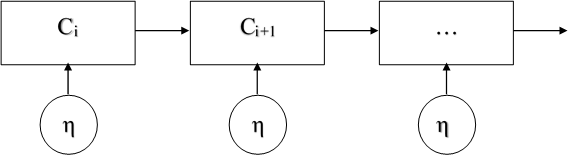
\includegraphics[scale=.7]{img/streamingprior.png}
\label{fig:streamingprior}

\end{center}
\caption{Học dòng với sự tăng cường tri thức tiên nghiệm}

\end{figure}
Sử dụng các quy ước và biểu diễn như ở phần \ref{subsec:streamingintro}. Khi có thêm tri thức tiên nghiệm $\eta$, xác suất hậu nghiệm ứng với thông tin từ $B-1$ minibatch xác định bởi
\begin{equation}
p(\Phi | C_1, C_2, ...,C_{B-1},\eta)
\end{equation}
Sau khi có thêm minibatch $C_B$, chúng ta cần tối ưu
\begin{equation}
p(\Phi | C_1,C_2,...C_{B-1},C_{B},\eta)
\end{equation}
Tiếp tục sử dụng phương pháp xấp xỉ, tuy nhiên tại đây, ở mỗi minibatch chúng ta tăng thêm lượng thông tin từ tri thức tiên nghiệm
\begin{equation}
p(\Phi | C_1,...,C_B,\eta) \approx q(\Phi | \eta)p(\Phi | \eta) = A(C,q_{B-1}(\Phi | \eta)).p(\Phi | \eta)
\end{equation}
Tiếp tục sử dụng biến đổi Bayes, ta được
\begin{equation}\label{eq:newstreaminggupdate2}
p(\Phi | C_1,...,C_B,\eta) \approx q(\Phi | \eta) p(\Phi | \eta) \propto [\prod_{b=1}^{B} A(C_b,p(\Phi | \eta))] p(\Phi | \eta)
\end{equation}
Công thức (\ref{eq:newstreaminggupdate2}) khác với công thức cũ (\ref{eq:oldstreamupdate}) ở lượng thông tin có từ prior $p(\Phi | \eta)$ được liên tục tăng cường sau mỗi mini-batch.\\
Khi sử dụng các phương pháp xấp xỉ, họ hàm mũ thường được sử dụng. Giả thiết khi đó:
\begin{equation}
 p (\Phi | \eta) \propto exp(\zeta_{0|\eta} T(\Phi | \eta))
\end{equation}
và
\begin{equation}
q_{b}(\Phi | \eta ) \propto exp(\zeta_{b|\eta} T(\Phi | \eta))
\end{equation}
Bây giờ, công thức học dòng trở thành:
\begin{equation}\label{eq:newstreamingupdate}
p (\Phi | C_1,...,C_B,\eta) \approx q(\Phi | \eta) \propto [\prod_{b=1}^{B} exp(\zeta_{0|\eta} + \sum_{b=1}^{B} \zeta_{b|\eta})]T(\Phi | \eta)
\end{equation}
Đối chiếu với công thức cập nhật ở (\ref{eq:oldstreamupdate}) cho dạng phân phối mũ:
\begin{equation}
p (\Phi | C_1,...,C_B,\eta) \approx [\prod_{b=1}^{B} exp(\zeta_{0|\eta} + \sum_{b=1}^{B} (\zeta_{b|\eta}-\zeta_{0|\eta})]T(\Phi | \eta)
\end{equation}
Ta nhận thấy rằng lượng thông tin có được từ tri thức tiên nghiệm $p(\Phi | \eta)$ không bị trừ đi trong mỗi minibatch, do đó sẽ tăng cường được vai trò của nó trong quá trình học dòng.
\subsection{Áp dụng phương pháp học dòng tăng cường tri thức tiên nghiệm cho mô hình LDA}
Phần này trình bày về phương pháp đưa tri thức từ vựng để sử dụng làm tri thức tiên nghiệm cho mô hình LDA, sau đó áp dụng phương pháp học dòng vừa đề xuất.
\subsubsection{Đưa tri thức từ vựng vào mô hình LDA}
Từ phần \ref{sub:wordknowledge}, ta đã có một số các tri thức về từ vựng. Sử dụng những tri thức này, chúng ta sẽ chuyển về dạng phân phối nhằm đưa vào tham số của phân phối Dirichlet $\eta$ của các từ trong $\beta$
\par 
\textbf{\textit{1. Tri thức từ các từ đặc trưng của chủ đề}}\\
Trong trường hợp này, chúng ta đã có tri thức về nhiều chủ đề, như vậy dạng của $\eta$ là một ma trận $K \times V $ với $K$ là số chủ đề, $V$ là kích thước từ vựng.
\begin{itemize}

\item Khởi tạo tất cả các giá trị của $\eta$ bằng một giá trị $\epsilon_0 < 1$. Mục đích của điều này để thể hiện các từ đều chưa được xác định rõ, khởi tạo mặc định bằng một giá trị nhỏ để đặc trưng cho tính thưa của các chủ đề.
\item Với các chủ đề đã xác định được từ đặc trưng seed-word, gán cho giá trị các từ này trong ma trận $\eta$ một giá trị hằng số $c > \epsilon$. Như vậy chúng ta đã nhấn mạnh vào việc các từ đặc trưng này sẽ có xác suất xuất hiện nhiều hơn trong chủ đề.
\end{itemize}
Với cách khởi tạo này, những chủ đề chưa biết sẽ được khởi tạo bằng một prior với các giá trị nhỏ, việc khởi tạo này tương ứng với việc sẵn sàng học ra các chủ đề ẩn chưa xác định của mô hình.
\par
\textbf{\textit{2. Tri thức từ luật Zipf's}}\\
Với luật Zipf's, chúng ta không có tri thức về các chủ đề cụ thể mà chỉ có một phân phối nền chung cho các từ của tập văn bản. Vì vậy dạng của $\eta$ sẽ là một vector $1\times V$ chung cho các chủ đề.
Việc khởi tạo cho $\eta$ được thực hiện như sau:
\begin{itemize}
\item Lấy hạng của các từ trong bảng xếp hạng tần số của các từ. Bảng xếp hạng tần số của các từ này được lấy từ các nghiên cứu của ngôn ngữ, hoặc có thể thực hiện thống kê trên bộ dữ liệu quan sát.
\item Gán các giá trị của $\eta$ theo công thức luật Zipf's mở rộng ở (\ref{eq:zipex}), giá trị hằng số trong công thức được gán bằng một giá trị nhỏ để đảm bảo tính thưa của phân phối các từ theo chủ đề. 
\end{itemize}
\subsubsection{Áp dụng phương pháp học dòng tăng cường tri thức vào LDA}
\label{sec:PartIII}
Sau khi có được tri thức tiên nghiệm từ $\eta$, chúng ta sẽ tăng cường nó vào quá trình học dòng thông qua công thức cập nhật đề xuất (\ref{eq:newstreaminggupdate2}).\\
Phân phối của các từ trong chủ đề $\beta$ không được tính trực tiếp, mà sẽ tính bằng xấp xỉ biến phân của nó $q(\beta | \eta) = Dir(\lambda | \eta)$.
Lúc này ta có thuật toán học dòng cho LDA như sau: 





\begin{algorithm}[H]
\begin{algorithmic}
\caption{Thuật toán học dòng tăng cường tri thức tiên nghiệm cho mô hình LDA}
\label{streamupdateLDA}
\REQUIRE{ Tri thức tiên nghiệm $\eta$, tham số $\alpha$, chuỗi các minibatch văn bản $C_1,C_2,...$}
\ENSURE{Dãy các xấp xỉ biến phân  $\lambda_1, \lambda_2,…$\\}
Khởi tạo : $\lambda_0 \leftarrow \eta$\\
\FOR {each mini-batch $C \in C_1,C_2,...$} 
\FOR{each document $d \in C$}
\STATE {$\Phi_{d} \leftarrow LocalInference(d,\lambda)$\\}
\ENDFOR\\
$\tilde{\lambda_b} \leftarrow \eta + \sum_{d \in C} \Phi_{dvk}n_{dv}$\\
$\lambda_{b} \leftarrow \lambda_{b-1}+\tilde{\lambda_{b}}$
\ENDFOR
\end{algorithmic}
\end{algorithm}
Trong mô hình học không có bổ sung tri thức:
\begin{algorithm}[H]
\begin{algorithmic}
\caption{Thuật toán học dòng \emph{không} tăng cường tri thức tiên nghiệm cho mô hình LDA}
\label{streamupdateLDAOld}
\REQUIRE{ Tri thức tiên nghiệm $\eta$, tham số $\alpha$, chuỗi các minibatch văn bản $C_1,C_2,...$}
\ENSURE{Dãy các xấp xỉ biến phân  $\lambda_1, \lambda_2,…$\\}
Khởi tạo : $\lambda_0 \leftarrow \eta$\\
\FOR {each mini-batch $C \in C_1,C_2,...$} 
\FOR{each document $d \in C$}
\STATE {$\Phi_{d} \leftarrow LocalInference(d,\lambda)$\\}
\ENDFOR\\
$\tilde{\lambda_b} \leftarrow  \sum_{d \in C} \Phi_{dvk}n_{dv}$\\
$\lambda_{b} \leftarrow \lambda_{b-1}+\tilde{\lambda_{b}}$
\ENDFOR
\end{algorithmic}
\end{algorithm}
Điểm khác biệt duy nhất giữa hai thuật toán học dòng này là thành phần học được từ mỗi minibatch $\tilde{\lambda_{b}}$. Trong khi mô hình học cũ không có thành phần tri thức tiên nghiệm $\eta$, từ đó thông tin ban đầu từ $\eta$ có thể rất tốt nhưng sẽ bị mất dần đi trong quá trình học. Ở cách cập nhật nhật mới $\eta$ luôn được bổ sung vào, do vậy tri thức tiên nghiệm được tăng cường, khi tri thức này có ý nghĩa thì nó sẽ luôn được duy trì trong quá trình học dòng.
\par
Hàm suy diễn cho văn bản $LocalInference(d,\lambda)$ dùng để tìm ra các tham số cho văn bản $d$. Ta sử dụng 3 phương pháp suy diễn như đã trình bày ở \ref{sub:infermethods} là Variant Bayes (VB), Frank-Wolfe (FW) và Online Frank-Wolfe (Online-FW). Ta tóm tắt lại các công thức suy diễn :\\
\textit{1. Suy diễn bằng variant Bayes}
\begin{algorithm}[H]
\begin{algorithmic}
\caption{LocalInfer-VB}
\label{variantBayes}
\REQUIRE{ văn bản $d$, tham số $\alpha,\lambda$}
\ENSURE{$\Phi$\\}
Khởi tạo : $\Phi$\\
\REPEAT
\STATE {$\gamma_{k} \leftarrow \alpha + \sum_{d_j}\Phi_{jk}d_{j}$}
\STATE {$\Phi_{jk} \propto exp(\psi(\gamma_k)).exp[\psi(\lambda_{kj}-\psi(\sum_{t}\lambda_{kt})]$}
\UNTIL{Hội tụ}\\
\end{algorithmic}
\end{algorithm}
\textit{2. Suy diễn bằng Frank - Wolfe}
 \begin{algorithm}[H]
\begin{algorithmic}
\caption{LocalInfer-FW}
\label{frankwolfeInfer}
\REQUIRE{ văn bản $d$, tham số $\lambda$}
\ENSURE{$\Phi$\\}
\STATE {Xấp xỉ $\beta \propto \lambda$ }\\
\STATE {Tính phân phối của các chủ đề  $\theta \leftarrow FW(\beta,d)$}\\
\STATE {$\Phi_{jk} \propto \theta_{k}\beta_{kj}$}
\end{algorithmic}
\end{algorithm} 
\textit{3. Suy diễn bằng Online Frank-Wolfe}
 \begin{algorithm}[H]
\begin{algorithmic}
\caption{LocalInfer-OFW}
\label{frankwolfeInfer}
\REQUIRE{ văn bản $d$, tham số $\alpha,\lambda$}
\ENSURE{$\Phi$\\}
\STATE {Xấp xỉ $\beta \propto \lambda$ }\\
\STATE {Tính phân phối của các chủ đề  $\theta \leftarrow OFW(\alpha,\beta,d)$}\\
\STATE {$\Phi_{jk} \propto \theta_{k}\beta_{kj}$}
\end{algorithmic}
\end{algorithm} 
\subsubsection{Vấn đề overfitting}
Overfitting xảy ra khi tham số mô hình học ra chỉ đúng với lượng dữ liệu học mà không có tính tổng quát cho bộ phận dữ liệu còn lại. Trở lại với thuật toán cập nhật ở thuật toán (\ref{streamupdateLDA}) ta có thể viết lại dưới dạng:
\begin{align}
\lambda_{b} \leftarrow b.\eta +  \sum_{C_i \in C}\sum_{d \in C_i} \Phi_{dvk}n_{dv}
\end{align}
Như vậy khi $b>>1$ thì $b.\eta >> 1$.
Thành phần $\eta$ sẽ chiếm vai trò rất lớn trong quá trình học ra $\lambda$, do vậy chất lượng của tri thức tiên nghiệm phải cao. Ngoài ra, để tránh overfitting, lượng thông tin học được từ dữ liệu cần phải lớn hơn lượng thông tin cung cấp từ prior.
Tức $\eta << \sum_{d \in C_i} \Phi_{dvk}n_{dv}$, do là nguyên nhân $\eta$ cần được khởi tạo bởi một giá trị nhỏ. \\
Tuy nhiên trong thực tế số lượng minibatch là nhỏ so với số lượng văn bản ( Số lượng minibatch =  Tổng số lượng văn bản / Số lượng văn bản trong một minibatch )nên lượng đóng góp do tri thức tiên nghiệm chỉ chiếm một phần trong tham số của mô hình. Do vậy tránh được vấn đề overfitting.
\newpage
\section{Thử nghiệm}
\label{sec:partIV}
Phần này trình bày về thử nghiệm đánh giá mô hình học dòng với tri thức tiên nghiệm tăng cường ( thuật toán (\ref{streamupdateLDA}))  và so sánh với mô hình học gốc không có sự tăng cường tri thức tiên nghiệm (thuật toán (\ref{streamupdateLDAOld})) trên mô hình LDA với 3 phương pháp suy diễn được trình bày ở phần \ref{sub:infermethods} gồm variant Bayes, Frank-Wolfe và Online - Frank Wolfe. Mức độ tốt của các mô hình được đánh giá bằng khả năng tổng quát hóa của mô hình chủ đề. Các đánh giá được thực hiện với 3 bộ dữ liệu Grolier, Nytimes, Pubmed.
\subsection{Phương pháp đánh giá }
Mục tiêu của học mô hình chủ đề là học ra các chủ đề ẩn trong dữ liệu, đồng thời tạo ra mô hình tổng quát cho các văn bản cho dữ liệu. Để đánh giá mức độ tổng quát, chúng ta sẽ tính khả năng tiên đoán của mô hình cho dữ liệu mới dựa trên thông số học được từ dữ liệu cũ.\\
Các từ trong mỗi văn bản dùng để test được chia ngẫu nhiên làm 2 phần $(tw_1,tw_2)$ với tỉ lệ $4:1$, xác suất xuất hiện của các từ trong $tw_2$ được tính toán dựa trên sự xuất hiện của các từ trong $tw_1$. Nếu xác suất này cao, chứng tỏ mô hình có tính dự đoán tốt và càng tổng quát.\\
Đặt D là tập văn bản được sử dụng để học ra các tham số mô hình $\beta$. Quá trình duy diễn văn bản cần test học ra tham số $\theta$ . Khi đó xác xuất dự đoán của văn bản tương ứng:
\begin{align}
p(tw_2 | D, tw_1) &= \int \int (\sum_{k=1}^{K} \theta_{k}\beta_{k,tw_2})p(\theta | tw_1,\beta)p(\beta|D)d\theta d\beta\\
&= \sum_{k=1}^{K}E(\theta_{k})E(\beta_{k,tw_2})
\end{align}
Chỉ số sử dụng để đánh giá khả năng tiên đoán của mô hình được gọi là \textbf\textit{Predictive Probability}. Trên thực tế, chúng ta sử dụng logarit của giá trị này \textit{log Predictive Probability}.
\par
Sau khi mỗi minibatch học xong, độ tổng quát được đánh giá lại. Việc so sánh giá trị này giữa các phương pháp học sẽ đưa ra đánh giá mô hình nào có khả năng tổng quát cao hơn.
\subsection{Dữ liệu thử nghiệm}
Thử nghiệm được thực hiện trên 3 bộ dữ liệu Grolier, Nytimes và Pubmed. Để mô phỏng cho việc học dòng, tập văn bản sẽ được chia thành các đoạn minibatch và đưa liên tục vào mô hình. Bảng sau đưa ra các thông số của bộ dữ liệu.
\begin{table}[H]
\begin{center}
\begin{tabular}{|l|l|l|}
\hline
& Kích thước từ vựng & Số lượng văn bản \\
\hline
Grolier & 15.276 & 23.044\\
\hline
Nytimes & 102.660 & 200.000 \\
\hline
Pubmed & 141.044 & 100.000\\
\hline 
\end{tabular}
\end{center}
\end{table}
\begin{itemize}
\item Bộ dữ liệu Grolier gồm các bài viết trong từ điển bách khoa của nhà xuất bản Grolier. [Nguồn ] gồm 23.044 văn bản với lượng từ vựng 15.276 từ
\item Bộ dữ liệu Nytimes gồm các bài viết từ hãng báo Newyork Times, [ Nguồn ]. Bộ dữ liệu sử dụng gồm 200.000 văn bản với 102.660 từ
\item Bộ dữ liệu Pubmed là các bài viết liên quan về sức khỏe - Thuộc trung tâm thông tin sinh học mỹ. Thử nghiệm sử dụng tập con gồm 100.000 văn bản với 141.044 từ vựng.
\end{itemize}
\subsection{Trích xuất tri thức tiên nghiệm}
Để có thể áp dụng được mô hình học tăng cường tri thức tiên nghiệm, chúng ta cần chọn ra được prior tin cậy và chất lượng. Như trình bày ở phần \ref{sub:wordknowledge} , ta có thể sử dụng tri thức về từ đặc trưng của chủ đề nhằm khởi tạo prior cho mô hình. Tuy nhiên những tri thức từ này thường khó thu thập và cần nhiều tri thức chuyên gia, vì vậy đồ án này chỉ thực hiện thử nghiệm theo phương án sử dụng luật Zipf's.
\subsubsection{Xử lí trên bộ dữ liệu Grolier và Nytimes}
Hai bộ dữ liệu này gồm các bài báo nói về chủ đề phổ thông, vì vậy sẽ gần với cấu trúc của một văn bản tiếng Anh thông thường. Bảng xếp hạng các từ sẽ được trích xuất ra từ bảng xếp hạng tần số các từ của tiếng Anh được thu thập từ trang http://www.wordfrequency.info/\textsuperscript{\cite{listfrequencyword}} \\
Việc trích xuất ra tham số tiên nghiệm $\eta$ được thực hiện với công thức luật Zipf's mở rộng (\ref{eq:zipex}), hệ số $q = 0.07$ và hằng số được đặt bằng $0.5$
\subsubsection{Xử lí trên bộ dữ liệu Pubmed}
Do bộ dữ liệu này liên quan tới chủ đề chuyên môn về sinh học, vì vậy tập các từ sẽ không theo quy luật xếp hạng của một văn bản thông thường. Để xếp hạng tần số các từ, ta cần thống kê lại tuần số xuất hiện của các từ trong tập dữ liệu, từ đó xếp hạng.
Sau khi có được bảng xếp hạng tần số các từ, việc chọn ra $\eta$ được thực hiện tiếp như trên bộ Grolier và Nytimes
\subsection{Các tham số cài đặt}
Kích thước các minibatch dữ liệu cho các tập dữ liệu được chia như sau
\begin{itemize}
\item Grolier : 500 văn bản
\item Nytimes : 10.000 văn bản
\item Pubmed: 5.000 văn bản
\end{itemize}
Số lượng chủ đề ẩn được đặt cố định $K = 100$ và tham số $\alpha = 0.01$  cho cả 3 bộ dữ liệu. Các lần chạy được thực hiện 5 lần và đưa ra giá trị trung bình. Riêng với suy diễn sử dùng Frank-Wolfe, hệ số $\alpha = 1$ ( thực tế được bỏ qua trong quá trình học)
\subsection{Kết quả và đánh giá}
Việc đánh giá sẽ được thực hiện lần lượt cho các bộ dữ liệu với cả 3 phương pháp suy diễn. Trong đó:
\begin{itemize}
\item Trục $x$ (Minibatch) là chiều tăng theo số minibatch nhận được
\item Trục $y$ (Log predictive probability) là giá trị đánh giá khả năng tiên đoán của mô hình
\end{itemize}
Đường biểu diễn kết quả cho phương pháp giữ tri thức tiên nghiệm được kí hiệu là $KP$ (Keeping prior)là đường với chấm tròn. Đường biểu diễn kết quả cho phương pháp cũ không tăng cường tri thức tiên nghiệm được gọi là $Origin$, là đường với ô vuông.
\newpage
\subsubsection{Kết quả đánh giá cho bộ dữ liệu Grolier}

\begin{figure*}[h!]
\begin{center}
\pgfplotstableread[col sep = comma]{data/gro_fw.csv}\mydata
\begin{tikzpicture}
  \begin{axis}[
   width=0.85\textwidth,
   height=0.55\textwidth,   
   legend entries={KP,Origin},
   legend style={
	at={(1.03,0.5)},
	anchor=west
   },
   xlabel={ Minibatch (x1000)},
   ylabel={Log predictive probability}],  
   ]
    \addplot table[x index = {0}, y index = {1}]{\mydata};
    \addplot table[x index = {0}, y index = {2}]{\mydata};
  \end{axis}
\end{tikzpicture}

\caption{Đánh giá học dòng sử dụng suy diễn FW với Grolier}
\label{fig:gro_fw}
\end{center}
\end{figure*}
\begin{figure*}[h!]
\begin{center}
\pgfplotstableread[col sep = comma]{data/gro_ofw.csv}\mydata
\begin{tikzpicture}
  \begin{axis}[
   width=0.85\textwidth,
   height=0.55\textwidth,  
   legend entries={KP,Origin},
   legend style={
	at={(1.03,0.5)},
	anchor=west
   }, 
   xlabel={ Minibatch (x1000)},
   ylabel={Log predictive probability}],  
    ]
    \addplot table[x index = {0}, y index = {1}]{\mydata};
    \addplot table[x index = {0}, y index = {2}]{\mydata};

  \end{axis}
\end{tikzpicture}
%}
%\end{minipage}
\caption{Đánh giá học dòng sử dụng suy diễn OFW với Grolier}
\label{fig:gro_ofw}
\end{center}
\end{figure*}
\begin{figure*}[h!]
\begin{center}
%\begin{minipage}{\linewidth}
%\subfloat[FW]{
%\label{FW}
\pgfplotstableread[col sep = comma]{data/gro_vb.csv}\mydata
\begin{tikzpicture}
  \begin{axis}[
   width=0.85\textwidth,
   height=0.55\textwidth, 
   legend entries={KP,Origin},
   legend style={
	at={(1.03,0.5)},
	anchor=west
   },
   xlabel={ Minibatch (x1000)},
   ylabel={Log predictive probability}],  
  ]
    \addplot table[x index = {0}, y index = {1}]{\mydata};
    \addplot table[x index = {0}, y index = {2}]{\mydata};

  \end{axis}
\end{tikzpicture}
%}
%\end{minipage}
\caption{Đánh giá học dòng sử dụng suy diễn VB với Grolier}
\label{fig:gro_vb}
\end{center}
\end{figure*}
\par Kết quả cho bộ Grolier được thể hiện ở các hình \ref{fig:gro_fw},\ref{fig:gro_ofw} và \ref{fig:gro_vb}. Khả năng tiên đoán của mô hình học dòng có tăng cường prior ($KP$) tốt hơn hẳn so với mô hình nguyên gốc ($Origin$) khi sử dụng suy diễn FW (hình \ref{fig:gro_fw}), và cũng tốt hơn khi sử dụng $OFW$ (hình \ref{fig:gro_ofw}). Tuy nhiên với suy diễn $VB$, thì phương pháp mới $KP$ lại kém một chút nhưng không đáng kể so với phương pháp cũ (hình \ref{fig:gro_vb}). Nhưng mặt khác giá trị đánh giá khả năng tổng quát của $FW$ và $OFW$ đạt tới gần $-36.000$ trong khi $VB$ chỉ đạt $-38.000$, nói cách khác, thuật toán sử dụng $VB$ cho ra kết quả kém hơn so với việc sử dụng $FW$ và $OFW$. Với riêng suy diễn $OFW$, về những minibatch cuối, kết quả 2 phương pháp có xu hướng gần bằng nhau. 
\newpage
\subsubsection{Kết quả đánh giá cho bộ dữ liệu Nytimes}

\begin{figure*}[h!]
\begin{center}
%\begin{minipage}{\linewidth}
%\subfloat[FW]{
%\label{FW}
\pgfplotstableread[col sep = comma]{data/nyt_fw.csv}\mydata
\begin{tikzpicture}
  \begin{axis}[
   width=0.85\textwidth,
   height=0.55\textwidth,    
   legend entries={KP,Origin},
   legend style={
	at={(1.03,0.5)},
	anchor=west
	},
  xlabel={ Minibatch (x10.000)},
  ylabel={Log predictive probability}],  
    ]
    \addplot table[x index = {0}, y index = {1}]{\mydata};
    \addplot table[x index = {0}, y index = {2}]{\mydata};

  \end{axis}
\end{tikzpicture}
%}
%\end{minipage}
\caption{Đánh giá học dòng sử dụng suy diễn FW cho Nytimes}
\label{fig:nyt_fw}
\end{center}
\end{figure*}
\begin{figure*}[h!]
\begin{center}
%\begin{minipage}{\linewidth}
%\subfloat[FW]{
%\label{FW}
\pgfplotstableread[col sep = comma]{data/nyt_ofw.csv}\mydata
\begin{tikzpicture}
  \begin{axis}[
   width=0.85\textwidth,
   height=0.55\textwidth,   
 legend entries={KP,Origin},
legend style={
at={(1.03,0.5)},
anchor=west
},
    xlabel={ Minibatch (x10.000)},
   ylabel={Log predictive probability}],  
    ]
    \addplot table[x index = {0}, y index = {1}]{\mydata};
    \addplot table[x index = {0}, y index = {2}]{\mydata};

  \end{axis}
\end{tikzpicture}
%}
%\end{minipage}
\caption{Đánh giá học dòng sử dụng suy diễn OFW cho Nytimes}
\label{fig:nyt_ofw}
\end{center}
\end{figure*}
\begin{figure*}[h!]
\begin{center}
%\begin{minipage}{\linewidth}
%\subfloat[FW]{
%\label{FW}
\pgfplotstableread[col sep = comma]{data/nyt_vb.csv}\mydata
\begin{tikzpicture}
  \begin{axis}[
   width=0.85\textwidth,
   height=0.55\textwidth,   
 legend entries={KP,Origin},
legend style={
at={(1.03,0.5)},
anchor=west
},
    xlabel={ Minibatch (x10.000)},
   ylabel={Log predictive probability}],  
%   xmin = 0,
%    xmax = 20,
%   ymin = -42000,
%   ymax = -30000,
    ]
    \addplot table[x index = {0}, y index = {1}]{\mydata};
    \addplot table[x index = {0}, y index = {2}]{\mydata};

  \end{axis}
\end{tikzpicture}
%}
%\end{minipage}
\caption{Đánh giá học dòng sử dụng suy diễn VB cho Nytimes}
\label{fig:nyt_vb}
\end{center}
\end{figure*}
Kết quả được thể hiện ở các hình \ref{fig:nyt_fw}, \ref{fig:nyt_ofw} và \ref{fig:nyt_vb}. Chúng ta có thể thấy kết quả có phần tương tự như ở bộ Grolier.\\
Khả năng tổng quát của phương pháp mới $KP$ vẫn vượt trội so với phương pháp cũ $Origin$ khi sử dụng suy diễn $FW$ và cao hơn rõ rệt khi sử dụng suy diễn $OFW$. Ở bộ dữ liệu này ta không thấy được sự khác biệt về chất lượng giữa 2 phương pháp khi sử dụng suy diễn $VB$, song kết quả với suy diễn sử dụng $VB$ ( đạt $-43.000$ ) vẫn kém hơn $FW$ và $OFW$ ($-42.000$). Do vậy khả năng tổng quát của mô hình khi sử dụng suy diễn $FW$ và $OFW$ của mô hình mới đạt kết quả tốt là có ý nghĩa hơn.\\ Chúng ta còn thấy thêm ở minibatch đầu tiên, phương pháp mới $KP$ cho chất lượng mô hình nhanh chóng được đẩy lên cao hơn so với phương pháp cũ ( hình \ref{fig:nyt_ofw}).
\newpage
\subsubsection{Kết quả thử nghiệm với bộ dữ liệu Pubmed}
\begin{figure*}[ht]
\begin{center}
%\begin{minipage}{\linewidth}
%\subfloat[FW]{
%\label{FW}
\pgfplotstableread[col sep = comma]{data/pub_fw.csv}\mydata
\begin{tikzpicture}
  \begin{axis}[
   width=0.85\textwidth,
   height=0.55\textwidth,   
legend entries={KP,Origin},
legend style={
at={(1.03,0.5)},
anchor=west
},
    xlabel={ Minibatch (x5.000)},
   ylabel={Log predictive probability}],  
    ]
    \addplot table[x index = {0}, y index = {1}]{\mydata};
    \addplot table[x index = {0}, y index = {2}]{\mydata};

  \end{axis}
\end{tikzpicture}
%}
%\end{minipage}
\caption{Đánh giá học dòng sử dụng suy diễn FW cho Pubmed}
\label{fig:pub_fw}
\end{center}
\end{figure*}
\begin{figure*}[h!]
\begin{center}
%\begin{minipage}{\linewidth}
%\subfloat[FW]{
%\label{FW}
\pgfplotstableread[col sep = comma]{data/pub_ofw.csv}\mydata
\begin{tikzpicture}
  \begin{axis}[
   width=0.85\textwidth,
   height=0.55\textwidth,   
legend entries={KP,Origin},
legend style={
at={(1.03,0.5)},
anchor=west
},
    xlabel={ Minibatch (x5.000)},
   ylabel={Log predictive probability}],  
   ]
    \addplot table[x index = {0}, y index = {1}]{\mydata};
    \addplot table[x index = {0}, y index = {2}]{\mydata};

  \end{axis}
\end{tikzpicture}
%}
%\end{minipage}
\caption{Đánh giá học dòng sử dụng suy diễn OFW cho Pubmed}
\label{fig:pub_ofw}
\end{center}
\end{figure*}
\begin{figure*}[h!]
\begin{center}
%\begin{minipage}{\linewidth}
%\subfloat[FW]{
%\label{FW}
\pgfplotstableread[col sep = comma]{data/pub_vb.csv}\mydata
\begin{tikzpicture}
  \begin{axis}[
   width=0.85\textwidth,
   height=0.55\textwidth,   
legend entries={KP,Origin},
legend style={
at={(1.03,0.5)},
anchor=west
},
    xlabel={ Minibatch (x5.000)},
   ylabel={Log predictive probability}],  
    ]
    \addplot table[x index = {0}, y index = {1}]{\mydata};
    \addplot table[x index = {0}, y index = {2}]{\mydata};

  \end{axis}
\end{tikzpicture}
%}
%\end{minipage}
\caption{Đánh giá học dòng sử dụng suy diễn VB cho Pubmed}
\label{fig:pub_vb}
\end{center}
\end{figure*}
\par Kết quả được thể hiện ở các hình \ref{fig:pub_fw}, \ref{fig:pub_ofw}, \ref{fig:pub_vb}. Các kết quả vẫn chung đặc điểm với 2 bộ Grolier và Nytimes:\\
Kết quả với suy diễn $FW$ cho thấy mô hình mới cho khả năng tổng quát cao hơn so với mô hình gốc ban đầu. Điều tương tự cũng xảy ra khi sử dụng suy diễn $OFW$ tuy nhiên kết quả không có sự chênh lệch quá lớn, và càng về cuối, 2 kết quả lại càng gần. Ở bộ Pubmed, kết quả của 2 phương pháp khi sử dụng $VB$ là gần như giống nhau song hiệu quả kém hơn $FW$ cùng $OFW$ ở mặt chỉ số đánh giá ($-44.000 $ so với $-42.000$).\\
Kết quả của phương pháp mới ngay từ những minibatch đầu tiên vẫn có xu hướng cao và gia tăng nhan hơn so với phương pháp cũ.
\newpage
\subsection{Nhận xét chung}
Chúng ta có thể thấy qua các kết quả từ 3 bộ dữ liệu Grolier, Nytimes và Pubmed: 
\begin{enumerate}
\item Chất lượng tiên đoán ( tổng quát) của phương pháp học dòng có tăng cường tri thức ($KP$) là cao hơn so với phương pháp học dòng cũ khi sử dụng suy diễn $FW$ và $OFW$.
\item Chất lượng tiên đoán của hai phương pháp là gần như nhau khi sử dụng suy diễn $VB$
\item Chất lượng tiên đoán từ những minibatch đầu tiên của phương pháp mới là cao và tăng nhanh hơn so với phương pháp cũ.
\item Khi càng nhiều dữ liệu, chất lượng đánh giá của 2 phương pháp có xu hướng tiến gần về nhau.
\end{enumerate}
Chúng ta có thể giải thích điều này như sau:\\
\begin{itemize}
\item Việc sử dụng thêm tri thức từ vào mô hình sẽ làm gia tăng chất lượng tổng quát của mô hình do mô hình có thêm những thông tin về đặc trưng của dữ liệu.
\item Ở những minibatch đầu tiên, khi thông tin từ dữ liệu chưa có nhiều, việc bổ sung thông tin từ tri thức từ càng quan trọng để tăng khả năng dự đoán.
\item Khi dữ liệu càng nhiều, lượng thông tin từ dữ liệu là đủ lớn để có thể bao chứa được thông tin từ tri thức tiền nghiệm. Có thể hiểu mô hình đã học ra được tri thức tiên nghiệm đặc trưng cho dữ liệu khi nhận được lượng thông tin đủ lớn.
\item Khả năng tổng quát hóa khi sử dụng suy diễn $FW, OFW$ là cao hơn khi sử dụng suy diễn $VB$ bởi không gian tìm kiếm của $FW, OFW$ rộng hơn, không sử dụng miền biến phân như suy diễn $VB$. Ngoài ra $FW, OFW$ đã được chứng minh tốc độ hội tụ đảm bảo hơn so với VB.\textsuperscript{\cite{dualonline}}
\end{itemize}
Việc kết quả của phương pháp học dòng mới không gia tăng được kết quả cho mô hình LDA khi sử dụng suy diễn $VB$ cũng thể hiện được phương pháp mới không có hiệu quả cho tất cả các mô hình cùng các biện pháp học dòng. Song kết quả trong những trường hợp xấu này cũng không thay đổi đáng kể.


\newpage
\section{Kết luận}
\label{sec:conclusion}
\subsection{Tổng kết kết quả đạt được trong đồ án}
Đồ án này đã thực hiện được việc sau: 
\begin{itemize}
\item Đưa ra vấn đề cần bổ sung tri thức từ vào quá trình học dòng cho mô hình LDA.
\item Đưa ra phương pháp học dòng chung có tăng cường tri thức tiên nghiệm.
\item Áp dụng phương pháp học dòng sử dụng tri thức tiên nghiệm về từ vào mô hình LDA.
\item Thực hiện các thử nghiệm đánh giá về chất lượng tổng quát hóa của mô hình học dòng sau khi có sử dụng tri thức từ vựng. Các kết quả trên các bộ dữ liệu thử nghiệm cho thấy mô hình học dòng với phương pháp tăng cường tri thức cho chất lượng cao hơn so với mô hình học dòng cũ không tăng cường tri thức từ.
\end{itemize}

\subsection{Những hướng tìm hiểu trong tương lai}
Đồ án này hiện chỉ đề cập tới tri thức về từ vựng với hai dạng: các từ đặc trưng của chủ đề và sử dụng luật Zipf's. Trong khi còn có nhiều tri thức bên ngoài khác như mối quan hệ về ngữ nghĩa giữa các từ trong ngôn ngữ ( WordNet). Việc trích xuất ra tri thức tiên nghiệm dưới dạng phân phối từ tri thức bên ngoài một cách hiệu quả cũng cần phải quan tâm. Ngoài ra đồ án hiện mới áp dụng cho mô hình học dòng LDA. Vì vậy cần có một số hướng tìm hiểu để phát triển phương pháp học dòng này:
\begin{itemize}
\item Tìm cách áp dụng thêm nhiều tri thức bên ngoài để đưa vào mô hình.
\item Tìm cách chuyển đổi tri thức bổ sung về dạng tri thức tiên nghiệm cho mô hình học dòng một cách hiệu quả.
\item Áp dụng cho nhiều mô hình học dòng khác.
\end{itemize}
\newpage
\section{Tài liệu tham khảo}
\label{sec:partVII}
\bibliographystyle{plain}
\bibliography{ref}{}
%\printbibliography
\end{document}